\section{Funktionen}
Eine Funktion $f: D \rightarrow W$ ist eine Abbildung, in der jedes Element aus
$D$ einem Element aus $W$ zugeordnet wird. $D$ ist der \underline{Definitionsbereich}
(Bereich der gültigen Eingaben) und $W$ der \underline{Wertebereich}
(Bereich der gültigen Ausgaben).

Bild von D: $f(D) = \{ f(x) \, | \, x \in D \}$ (Muss nicht gleich $W$ sein!)

Urbild von $V \subset W$: $f^{-1}(V) = \{ x \in D \, | \, f(x) \in V \}$\\
$ y = f(a) +(x-a)\cdot f'(x)$ da $f'(x) = \frac{f(x)-f(a)}{x-a}$

\subsection{Injektiv, surjektiv, bijektiv}
\subsubsection{Injektiv}\index{injektiv}
Sei $f: M \rightarrow N$, $f$ ist injektiv, wenn folgendes gilt:
\begin{itemize}
	\item $\forall x_1, x_2 \in M: x_1 \neq x_2 \Rightarrow f(x_1) \neq f(x_2)$
	\item $\forall x_1, x_2 \in M: f(x_1) = f(x_2) \Rightarrow x_1 = x_2$
	\item $\forall y \in N: \exists !x \in M: f(x) = y \lor \lnot(\exists x \in M: f(x) = y)$: wenn zu jedem $y \in N$ höchstens (genau eins oder keins) ein $x \in M$ existiert mit $f(x) = y$
\end{itemize}

%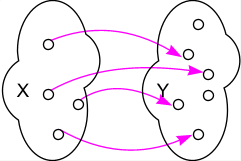
\includegraphics[scale=0.5]{injektiv.png}

\paragraph{Injektivität zeigen}
Injektiv wird meist direkt über die zweite Eigenschaft gemacht oder per Wiederspruchsbeweis (indirekter Beweis) mittels der ersten Eigenschaft bewiesen.

\paragraph{Eigenschaften}
\begin{itemize}
	\item Die Gleichung $f(x) = y$, $f$ ist injektiv und $y$ gegeben, verfügt über eine oder keine Lösung für $x$
	\item Eine \textit{stetige reelwertige} Funktion auf einem \textit{reelen Intervall} ist genau dann \underline{injektiv}, wenn sie in ihrem gesamten Definitionsbereich \textit{streng monoton} steigend oder fallend ist.
	\item Sind die beiden Funktionen $g, f$ injektiv, so ist die \underline{Komposition} $g \circ f$ ebenfalls injektiv
	\item Ist $g \circ f$ injektiv, so ist $f$ injektiv
	\item $f: M \rightarrow N$ ist injektiv, wenn es die \underline{links inverse} Funktion $g: N \rightarrow M$ gibt, so dass $g \circ f = \id_M$
\end{itemize}

\subsubsection{Surjektiv}\index{surjektiv}
Sei $f: M \rightarrow N$, $f$ ist surjektiv, wenn folgendes gilt:
\begin{align*}
\forall y \in N: \exists x \in M: f(x) = y
\end{align*}
Wenn also für jedes Element aus $N$ mindestens ein (können auch mehr sein) Element in $M$ gibt, dass auf das Element aus $N$ zeigt.

%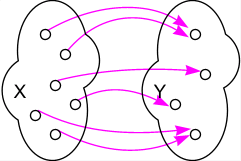
\includegraphics[scale=0.5]{surjektiv.png}

\paragraph{Eigenschaften}
\begin{itemize}
	\item Die Gleichung $f(x) = y$, $f$ ist surjektiv und $y$ gegeben, verfügt über eine oder mehrere Lösungen für $x$.
	\item Sind die Funktionen $f: A \rightarrow B$ und $g: B \rightarrow C$ surjektiv, so ist die \underline{Komposition} $g \circ f: A \rightarrow C$ auch surjektiv
	\item Ist $g \circ f$ surjektiv, so folgt, dass $g$ surjektiv ist
	\item $f: A \rightarrow B$ ist genau dann surjektiv, wenn $f$ ein \underline{rechtes Inverse} hat, also $g: B \rightarrow A$ mit $f \circ g = \id_B$
\end{itemize}

\subsubsection{Bijektiv}\index{bijektiv}
Eine Funktion ist bijektiv, wenn sie injektiv und surjektiv ist.

%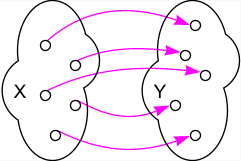
\includegraphics[scale=0.5]{bijektiv.png}
\vspace{-0.5cm}
\paragraph{Eigenschaften}
\begin{itemize}
	\item Es gelten die Eigenschaften von Injektivi. und Surjektivi.
	\item Die Gleichung $f(x) = y$, $f$ ist bijektiv und $y$ gegeben, verfügt über genau eine Lösung für $x$
	\item Sind die Funktionen $f: A \rightarrow B$ und $g: B \rightarrow C$ bijektiv, dann ist auch die \underline{Komposition} $g \circ f: A \rightarrow C$ bijektiv.
	\item Ist $g \circ f$ bijektiv, dann ist $f$ injektiv und $g$ surjektiv
\end{itemize}

\subsection{Absolutbetrag}
\begin{itemize}
	\item $|x| = \max(x, -x)$ oder 
	$\begin{array}{l}
		x \geq 0 \Rightarrow |x| = x \\
		x < 0 \Rightarrow |x| = -x
	\end{array}$
	\item $|x \cdot y| = |x| \cdot |y|$
	\item $|x + y| \leq |x| + |y|$
	\item $|x - a| < \epsilon \; \Leftrightarrow \;  -\epsilon < x- a < \epsilon \; \Leftrightarrow \; a - \epsilon < x < a + \epsilon$
	\item $|x - a| \Leftrightarrow |a - x|$
\end{itemize}

\subsection{Monotonie}
Die Funktion $f$ ist\ldots
\begin{description}
	\item[monoton steigend,] falls: $x_1 < x_2 \Rightarrow f(x_1) \leq f(x_2)$
	\item[streng monoton steigend,] falls: $x_1 < x_2 \Rightarrow f(x_1) < f(x_2)$
	\item[monoton fallend,] falls: $x_1 < x_2 \Rightarrow f(x_1) \geq f(x_2)$
	\item[streng monoton fallend,] falls: $x_1 < x_2 \Rightarrow f(x_1) > f(x_2)$
\end{description}

\subsubsection{Monotonie und Differenzial (Ableitung)}\index{monoton}
Ist $f$ auf dem Intervall $I$ differenzierbar, so gilt
\begin{itemize}
	\item $f'(x) > 0 \; \forall x \in I \Rightarrow f$ streng monoton steigend
	\item $f'(x) \geq 0 \; \forall x \in I \Leftrightarrow f$ monoton steigend
	\item $f'(x) < 0 \; \forall x \in I \Rightarrow f$ streng monoton fallend
	\item $f'(x) \leq 0 \; \forall x \in I \Leftrightarrow f$ monoton fallend
\end{itemize}
